\chapter*{Literature Review}
\addcontentsline{toc}{chapter}{Literature Review}

Related works of SSL are categorized into two sections, the traditional SSL methods and the DL based SSL approaches.

\section*{Review of Traditional SSL Methods}
\addcontentsline{toc}{section}{Review of Traditional SSL Methods}

Traditional Sound Source Localization (SSL) methods primarily rely on mathematical modeling of geometric and statistical principles. These approaches employ a variety of techniques to estimate the locations of sound sources within an environment. These foundational methods have established foundations for more sophisticated SSL techniques and remain crucial in various audio signal processing applications.

A typical traditional SSL method is the Time Difference of Arrival (TDOA) \cite{knapp_generalized_1976}. It positions the spatial location of a sound source by measuring the time differences of the sound signal arrival time between each microphone in a microphone array. With two microphones, the TDOA method can position the degree of arrival (DoA) of the sound source relative to the receiver, while three or more microphones can position the DoA and distance by triangulate positioning. TDOA methods have been progressively improved over the decades to adapt to various scenarios such as when the number of microphones is limited \cite{liu_arbitrary_2019} or when sound wave transmission mediums are different \cite{carevic_detection_2007}. Combining the TDOA method with other statistical models is also a research trend, combined with Generalized Cross-Correlation (GCC) \cite{chung_sound_2022} as an example. However, multiple research claimed that the TDOA method is limited when encountering situations such as high noise levels, low noise-signal ratio, and reverberant environment \cite{tachioka_method_2017} \cite{hao_network_2020}.

Another widely used classical algorithm is beamforming \cite{van_veen_beamforming_1988}. By employing microphone arrays to enhance signals coming from specific directions while suppressing signals from other directions, it scans all possible directions, and the direction with the maximum gain (main lobes) is estimated as the direction of the sound source. As another classical SSL approach, beamforming was utilized for various purposes. Based on beamforming methods, researchers proposed effective solutions to blind sound source separation based on geometric beam-forming \cite{parra_geometric_2002}. It was also proven to have the potential to be applied to robotic perception \cite{valin_localization_2004}. However, there is also a concern about the beamforming algorithm's performance in complex situations, including localizing non-stationary background noise \cite{comminiello_beamforming_2013}, and reverberant environment \cite{noh_dereverberation_2020}.

\begin{figure}[H]
    \centering
    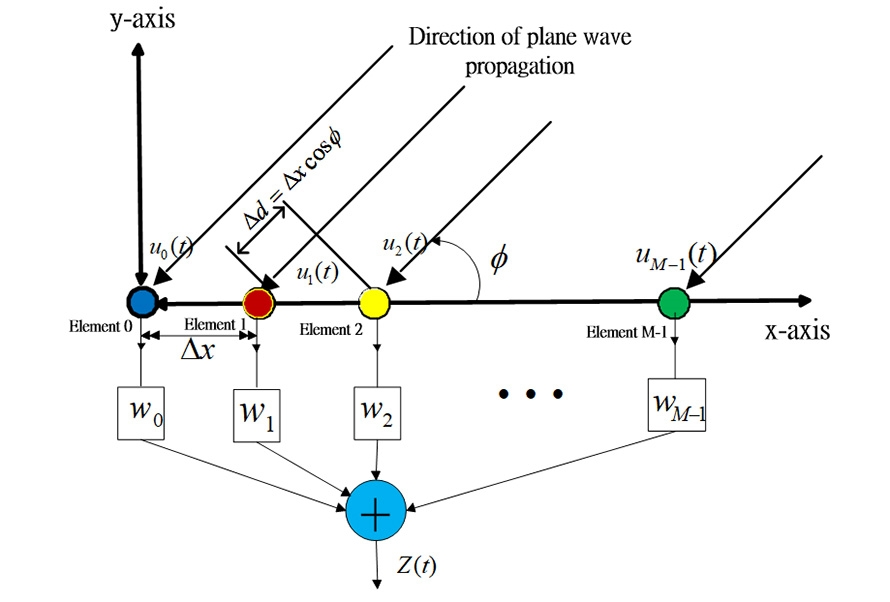
\includegraphics[width=0.4\linewidth]{figures/Explain_beamforming.png}
    \caption{Beamforming Utilizes Phase Shift to Enhance the Signal from the Scanned Direction}
\end{figure}


\section*{Review of Deep-Learning Based SSL Methods}
\addcontentsline{toc}{section}{Review of Deep-Learning Based SSL Methods}

With advancements in GPU technology and its computational capabilities during the last decade, the growing complexity of DNN architecture provides possibilities to improve the accuracy and robustness of the SSL. Recent studies demonstrate the robustness of DL-based SSL algorithms under noisy and reverberant environments \cite{wang_robust_2018} \cite{zhang_deep_2017} \cite{lee_sound_2020} \cite{ma_exploiting_2017}. The robustness of these algorithms while handling complex circumstances enables them to be deployed in a wider range of applications, with Unmanned Aerial Vehicle (UAV) \cite{wang_deep-learning-assisted_2022} as an example.

Most of the DL-based approaches for SSL purposes involve five stages: pre-processing, encoding, hidden layer processing, decoding, and post-processing.

Pre-processing refers to the data processing sequence before entering the DNN, usually referring to the feature extraction algorithm that directly handles the original sound signal, which is the amplitude-time sequential data. For an audio signal processing task, feature extraction usually maps the time-domain signal to the frequency domain. A significant number of machine-learning-based methods utilize the Mel-Frequency Cepstral Coefficients (MFCCs) method, such as \cite{di_applicability_2023} \cite{nsalo_kong_underwater_2024} \cite{palaniappan_comparative_2014} \cite{wang_research_2024}, for frequency-domain information extraction and the purpose of comprehending the human speaking sound. The Fourier Transform (FT), as part of the MFCCs method, projects the sound signal from the time domain to the frequency domain, allowing a more detailed analysis of the frequency features. Another commonly employed feature extraction technique is the Short-Time Fourier Transform (STFT), which retains time-domain information by applying the Fourier Transform to each time frame instead of the entire sound signal segment. This results in a spectrogram in the time-frequency domain, including the information along the time sequence. The STFT has been increasingly utilized recently as feature extraction for DNN, with examples including \cite{tan_sound_2021} 
\cite{chakrabarty_multi-speaker_2019} \cite{pujol_beamlearning_2021} \cite{schymura_pilot_2021} \cite{niu_deep-learning_2019} \cite{liu_rolling_2016}, due to its unique ability to handle time-sequential information. Meanwhile, some studies suggest that eliminating the feature extraction process, allowing the DNN to process the original time-domain sound signal directly, may yield improved performance. TasNet \cite{luo_tasnet_2018}, as an important study that resolves the audio channel separation problem by directly inputting the original multi-channel input into the DNN.

\begin{figure}[h]
    \centering
    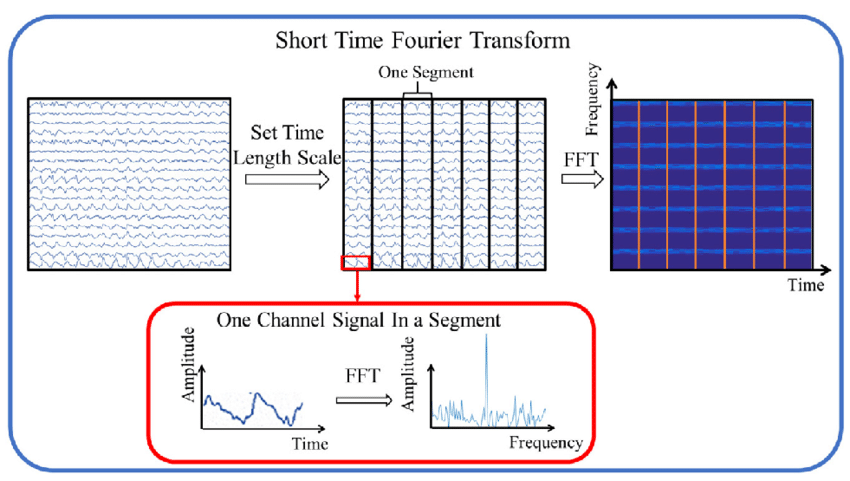
\includegraphics[width=0.75\linewidth]{figures/STFT_Explain.png}
    \caption{STFT: Applying Fourier Transform to Each Time Frame}
\end{figure}

The structures in the Deep Neural Networks (DNNs) consist of the encoder, hidden layer, and decoder. The fundamental concept of a DNN is to vectorize abstract features from the original dataset, construct a high-dimensional function (which predicts the expected output from input) described by the network itself, and compute the parameters in this function by repeated training using massive data with labeled ground truth. The training process usually refers to using gradient descent to find a local stable point in this function. In this context, the encoder refers to the mapping process from data to high-dimensional tensors for the DNN. The hidden layers serve as the prediction function. The decoder then translates the output tensors into the output required by the algorithm.

\begin{figure}[h]
    \centering
    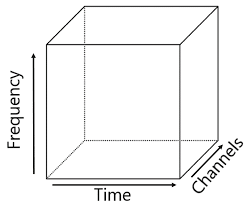
\includegraphics[width=0.25\linewidth]{figures/STFT_Tensor.png}
    \caption{The Time-Frequency Domain Spectrogram After STFT, Represented in the Form of A Tensor for Multi-Microphone-Channels Signal}
\end{figure}

\begin{figure}[h]
    \centering
    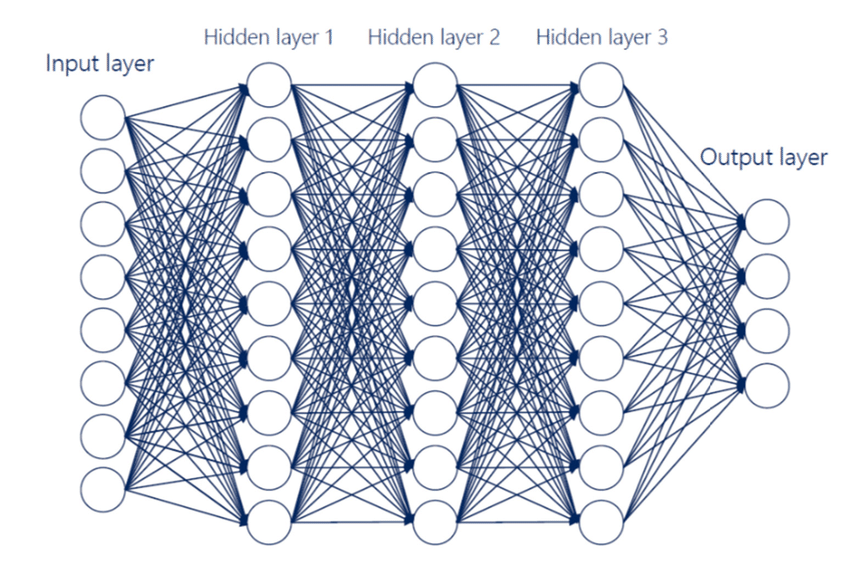
\includegraphics[width=0.5\linewidth]{figures/DNN_example2.png}
    \caption{A Simple Visualization of a Typical DNN}
\end{figure}

Whether post-processing is necessary depends on the specific settings of the SSL task. It is common for a DNN to directly output results, such as the locations of multiple sound sources in the form of a set of vectors or a time-sequence of coordinates representing the sound source's location, such as \cite{adavanne_sound_2019} \cite{zhang_mtf-crnn_2020} \cite{phan_robust_2016} \cite{kim_multi-scale_2022}. Alternatively, designing the DNN to output results to a traditional algorithm, known as post-processing, is another possible structural solution. SRP-DNN \cite{yang_srp-dnn_2022} is a suggestive example of utilizing DNN to predict the phase difference between a pair of microphones in a microphone array, which will be further constructed into a spatial spectrum for peak analysis, providing the result of the sound location.